\chapter{He Turned \$100k Into \$25M}

Todd Napola's interview gives us a compact case study in commercial real estate judgment. The mathematical content is not board work; it is deal arithmetic: a purchase price, a refinance value, a loan, returned capital, and continuing cash flow. We will follow the interview in its spoken order, because the order carries the lesson: first the promise, then mentorship, then the first risky property, then the obstacle of capital, the operating edge that makes deals repeatable, and finally the question of what remains if the bank account goes back to zero.

\section{The Promise: From Zero Cash to an Eight-Figure Portfolio}

The opening gives the result before it gives the mechanism. Todd is introduced as a South Florida commercial real estate operator who has built an eight-figure portfolio over roughly twenty-five years. The more useful fact, for our purposes, is the origin point: at twenty-five years old he put nearly all of his cash into a first property.

That first property is the small model of the whole chapter. It contains the pieces that later reappear at larger scale: control of an asset, operating work, financing, cash flow, and the willingness to look foolish before the result is visible. The later \$25 million shopping-center purchase matters because it shows the same pattern enlarged, not because it replaces the first story.

The host also previews a second claim that will matter later: capital is not always the scarce object. Todd will eventually argue that a sufficiently good deal attracts money; the hard part is finding the deal. We should hear that as a commercial judgment, not as a universal law.

\section{Mentorship as an Acquisition of Judgment}

The first question asks what Todd would tell a younger entrepreneur. His answer is short: find a mentor. But the story that follows shows what the word means in practice.

Todd hears Gary Rappaport speak at a real estate convention. Rappaport places business cards around the room and says that people will take them, but almost nobody will actually call. Todd treats that remark as a challenge. He waits outside the booth, introduces himself, explains that Gary's business is the work he wants to do, and asks whether he can visit the office and take him to lunch.

The mentor story is not just a story about access. It is a sequence of conversion:
\begin{enumerate}
\item a public offer becomes a card;
\item the card becomes a direct introduction;
\item the introduction becomes a concrete office visit;
\item the visit becomes a full day with someone far ahead in the field;
\item the day becomes an ongoing relationship.
\end{enumerate}

Todd later tells Gary that he has just closed a \$25 million deal. Gary answers that his own firm has just closed one for \$125 million, and frames it not as a put-down but as an instruction: keep going. The function of the mentor is partly technical and partly psychological. He changes the size of the numbers that feel normal:
\begin{equation}
\text{Todd's deal}=\$25\mathrm{M},
\qquad
\text{Gary's comparison}=\$125\mathrm{M}.
\end{equation}

\subsection{Question \& Answer}

\paragraph{Question.}
Why does asking for help so often fail, even when experienced people say they are willing to help?

\paragraph{Answer.}
Because the offer remains vague. Todd's story makes the offer operational. He does not merely admire the speaker, collect the card, and return home. He waits, asks for a specific meeting, travels, and stays in touch. Mentorship, in this interview, is not inspiration; it is repeated contact with someone whose judgment has already been tested in the exact business one wants to enter.

\section{The First Property: Risk, Repair, Refinance, Cash Flow}

Before Todd gives the numbers, the interview passes through a warning: do not count other people's money. He learned this around wealthy clients when he was young, and he connects it to the modern problem of social media. Many visible signs of wealth are not wealth. That warning clears away the false scoreboard before the first real risk appears.

The risk begins with the limits of commission income. Todd was a stockbroker in the 1990s and says he was doing well, but the income depended on transactions. If there was no trade, there was no commission. A week away meant a week with no new commission income. Real estate enters the story as an attempt to own something that could keep working even when he was not making trades.

At twenty-five, he buys his first property. He says he drains a six-figure bank account down to \$50. The stated purchase price is
\begin{equation}
P_{\mathrm{buy}}=\$575{,}000,
\qquad
C_{\mathrm{remaining}}=\$50.
\end{equation}

The property was not a passive bet. Todd says he re-tenanted it, cleaned it up, used friends as inexpensive labor, painted it, improved the appearance, and wrote leases for new tenants. The operating work is the bridge from the purchase number to the refinance number.

The transcript phrase around the refinance is slightly garbled, so we state the next quantity cautiously: Todd says the property was refinanced at an \$800,000 value and that he obtained a \$600,000 loan:
\begin{equation}
V_{\mathrm{refi}}=\$800{,}000,
\qquad
L_{\mathrm{refi}}=\$600{,}000.
\end{equation}

From those two stated numbers we can reconstruct a standard loan-to-value calculation:
\begin{equation}
\mathrm{LTV}
=
\frac{L_{\mathrm{refi}}}{V_{\mathrm{refi}}}
=
\frac{600{,}000}{800{,}000}
=
0.75
=
75\%.
\end{equation}
Todd does not use the term \(\mathrm{LTV}\) in the interview. We use it only as a clean way to read the financing arithmetic.

Todd then gives the payoff: the loan returned his money and closing costs, and beginning in January, seven months after the purchase, the property produced \$5,000 per month in free cash flow. Annualized, that monthly cash flow is
\begin{equation}
CF_{\mathrm{year}}
=
12\,CF_{\mathrm{month}}
=
12\cdot \$5{,}000
=
\$60{,}000.
\end{equation}
The annual figure is our arithmetic reconstruction. The transcript-backed figure is the monthly free cash flow.

\begin{table}
\centering
\begin{tabular}{ll}
\hline
Quantity & Amount or value \\
\hline
First property purchase price & \$575,000 \\
Cash left after purchase & \$50 \\
Refinance value, stated cautiously & \$800,000 \\
Refinance loan & \$600,000 \\
Inferred loan-to-value & 75\% \\
Monthly free cash flow & \$5,000 \\
Annualized free cash flow & \$60,000 \\
\hline
\end{tabular}
\caption{The first-property numbers. The purchase price, refinance value, loan, and monthly free cash flow come from Todd's account; the loan-to-value and annualized cash flow are simple reconstructions.}
\end{table}

\begin{figure}
\centering
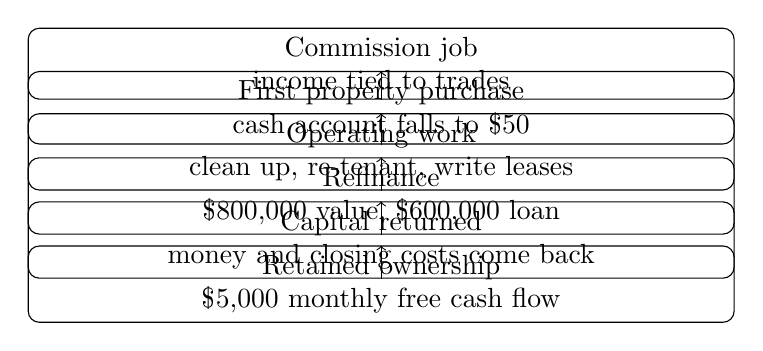
\begin{tikzpicture}[
  box/.style={draw, rounded corners, align=center, text width=0.72\linewidth, minimum height=0.62cm},
  node distance=0.56cm
]
\node[box] (job) {Commission job\\income tied to trades};
\node[box, below of=job] (buy) {First property purchase\\cash account falls to \$50};
\node[box, below of=buy] (work) {Operating work\\clean up, re-tenant, write leases};
\node[box, below of=work] (refi) {Refinance\\\$800,000 value, \$600,000 loan};
\node[box, below of=refi] (return) {Capital returned\\money and closing costs come back};
\node[box, below of=return] (cash) {Retained ownership\\\$5,000 monthly free cash flow};
\draw[->] (job) -- (buy);
\draw[->] (buy) -- (work);
\draw[->] (work) -- (refi);
\draw[->] (refi) -- (return);
\draw[->] (return) -- (cash);
\end{tikzpicture}
\caption{The first-property capital cycle, reconstructed from the interview rather than from a validated board diagram.}
\end{figure}

\subsection{Question \& Answer}

\paragraph{Question.}
How can a deal return the capital and still produce cash flow?

\paragraph{Answer.}
In Todd's telling, the answer is the sequence. The asset is controlled first. Then the operations are changed: tenants, appearance, leases, and management attention. Those changes support a higher refinance value. The loan then returns capital, while the property remains owned and continues to produce monthly free cash flow.

The safe arithmetic is limited but useful. The difference between the refinance value and purchase price is
\begin{align}
\Delta V
&=
V_{\mathrm{refi}}-P_{\mathrm{buy}} \\
&=
\$800{,}000-\$575{,}000 \\
&=
\$225{,}000.
\end{align}
Using the stated refinance value and loan, the implied equity after the refinance is
\begin{equation}
E_{\mathrm{after\ refi}}
=
V_{\mathrm{refi}}-L_{\mathrm{refi}}
=
\$800{,}000-\$600{,}000
=
\$200{,}000.
\end{equation}

These are not full profit calculations. The interview does not give renovation costs, original debt terms, closing costs, taxes, or the exact cash invested. The point is structural: operating improvement made refinancing possible, and refinancing changed a high-risk cash commitment into returned capital plus retained ownership.

\section{Books, Time Horizons, and One Property}

After the first-property sequence, the interview slows down. The host asks about the book that changed Todd's business life. Todd names Tony Robbins and emphasizes a time-horizon lesson: people overestimate what they can do in one year and underestimate what they can do in five.

He then broadens the claim. Reading, in his account, imports experience. A person with twenty-five or thirty years in a field can compress that experience into a book. Todd says he read sixty books in the prior year, and he treats books as a way to borrow other people's mistakes, patterns, and judgment.

That leads into Todd's own book on commercial real estate. The three lessons he names are deliberately practical:
\begin{itemize}
\item wealthy people in many industries tend to own real estate;
\item the right property type depends on the owner's life and available time;
\item beginners should start with a property they can understand and manage.
\end{itemize}

His strongest long-horizon claim is that one property can matter. If a person buys a property and pays it off over twenty to twenty-five years, Todd says that ownership can become retirement support. We preserve the claim as interview evidence, not as a universal theorem. The mechanism is long-term control:
\begin{equation}
\text{buy one understandable property}
\longrightarrow
\text{pay down debt}
\longrightarrow
\text{own the asset}
\longrightarrow
\text{future cash-flow support}.
\end{equation}

The pacing matters here. Todd does not leap straight from a first deal to a giant portfolio. He pauses on one durable unit of ownership: a property that fits the owner, can be learned, and can be held through time.

\section{The Capital Obstacle: The Deal Is Harder Than the Money}

The host then raises the beginner's objection: does one need a large amount of money before one can buy property? Todd answers with the sharpest maxim in the interview: go find a deal.

His example is intentionally extreme. He points to the Aventura Mall and estimates, roughly, that it may be worth \$3 billion. Then he asks us to imagine that someone offers it for \$1 billion, with the condition that the buyer must close the next morning. In Todd's telling, the capital would appear because the deal would be compelling.

We can write the illustrative arithmetic while keeping its status clear. The \$3 billion value is Todd's rough guess, and the \$1 billion price is hypothetical:
\begin{align}
V_{\mathrm{mall,guess}}&\approx \$3\mathrm{B},\\
P_{\mathrm{hypothetical}}&=\$1\mathrm{B},\\
\frac{P_{\mathrm{hypothetical}}}{V_{\mathrm{mall,guess}}}
&=
\frac{1}{3}
\approx 33.3\%.
\end{align}
The implied discount in the hypothetical is
\begin{equation}
1-\frac{1}{3}
=
\frac{2}{3}
\approx 66.7\%.
\end{equation}

The example separates two jobs:
\begin{itemize}
\item find a property whose price and economics make sense;
\item find capital once that opportunity can be shown.
\end{itemize}
Todd's claim is that the first job is often harder.

\begin{figure}
\centering
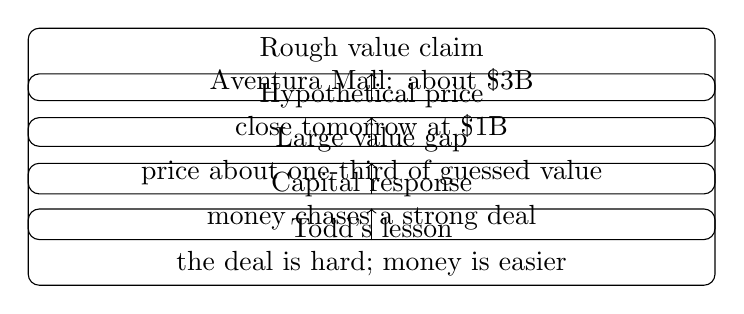
\begin{tikzpicture}[
  box/.style={draw, rounded corners, align=center, text width=0.70\linewidth, minimum height=0.62cm},
  node distance=0.58cm
]
\node[box] (value) {Rough value claim\\Aventura Mall: about \$3B};
\node[box, below of=value] (price) {Hypothetical price\\close tomorrow at \$1B};
\node[box, below of=price] (gap) {Large value gap\\price about one-third of guessed value};
\node[box, below of=gap] (capital) {Capital response\\money chases a strong deal};
\node[box, below of=capital] (lesson) {Todd's lesson\\the deal is hard; money is easier};
\draw[->] (value) -- (price);
\draw[->] (price) -- (gap);
\draw[->] (gap) -- (capital);
\draw[->] (capital) -- (lesson);
\end{tikzpicture}
\caption{The Aventura Mall hypothetical. The diagram preserves Todd's claim about deal quality while keeping the numbers marked as rough or hypothetical.}
\end{figure}

\subsection{Question \& Answer}

\paragraph{Question.}
If a beginner has no money and no credit, why does Todd say the deal is the scarce asset?

\paragraph{Answer.}
Because in his model, capital is attracted to asymmetry. A property that can be bought far below a credible value gives investors a reason to participate. The beginner may not contribute the full check; the beginner may contribute discovery, local knowledge, persistence, and a deal that makes sense.

This does not remove the need for judgment. It raises the standard for judgment. The task becomes learning a market well enough to recognize an opportunity that capital would rationally want.

\section{Operating Edge: Local Control and In-House Work}

The next question asks how Todd's company stands out in a competitive industry. His answer is not branding or personality. It is operating structure.

First, he keeps the geography tight. He says every property is within roughly 250 to 300 miles of where he is, close enough that he can drive to a property, understand the issue, have lunch, and return home for dinner:
\begin{equation}
R_{\mathrm{properties}}\approx 250\text{--}300\ \mathrm{miles}.
\end{equation}
That radius is a discipline. It defines the zone inside which market knowledge can stay personal and operational problems can be inspected directly.

Second, he keeps functions in-house: leasing, accounting, and property management. The pieces overlap. Managers know what other managers are doing. Tenants in one location can help fill vacancies in another. A nail salon tenant, in his example, may know another nail salon operator. The edge is not simply owning buildings; it is owning the information flow around the buildings.

\begin{figure}
\centering
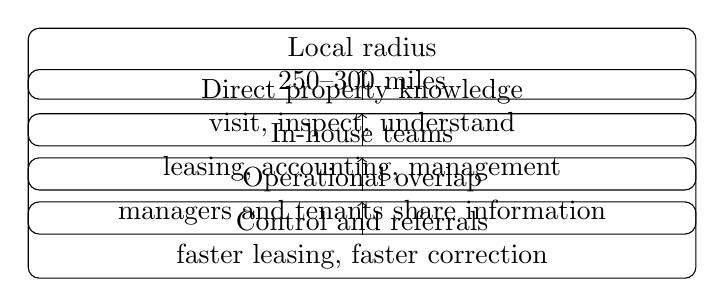
\begin{tikzpicture}[
  box/.style={draw, rounded corners, align=center, text width=0.68\linewidth, minimum height=0.62cm},
  node distance=0.56cm
]
\node[box] (radius) {Local radius\\250--300 miles};
\node[box, below of=radius] (knowledge) {Direct property knowledge\\visit, inspect, understand};
\node[box, below of=knowledge] (teams) {In-house teams\\leasing, accounting, management};
\node[box, below of=teams] (overlap) {Operational overlap\\managers and tenants share information};
\node[box, below of=overlap] (edge) {Control and referrals\\faster leasing, faster correction};
\draw[->] (radius) -- (knowledge);
\draw[->] (knowledge) -- (teams);
\draw[->] (teams) -- (overlap);
\draw[->] (overlap) -- (edge);
\end{tikzpicture}
\caption{Todd's operating edge: local control plus in-house information flow.}
\end{figure}

This section explains how the first-property pattern scales. The first property required direct work: clean it, re-tenant it, write leases. The company version is an organized machine for doing that kind of work repeatedly.

\section{Scale, Contrarian Timing, and the Reason to Keep Going}

Todd's largest discussed deal was a \$25 million acquisition of shopping-center property closed the previous December. The property had never been on the market. A father and son built it decades earlier, over roughly a ten-year period, and ownership later passed down through heirs. As ownership diluted, the situation became more complicated. Todd bought the property for \$25 million.

The stated scale is
\begin{equation}
P_{\mathrm{large\ deal}}=\$25\mathrm{M},
\qquad
A=165{,}000\ \mathrm{sq\ ft}.
\end{equation}
A simple descriptive calculation gives the purchase price per square foot:
\begin{equation}
\frac{\$25{,}000{,}000}{165{,}000}
\approx
\$151.52/\mathrm{sq\ ft}.
\end{equation}
This number is only a scale marker. The interview gives no rent roll, occupancy, debt terms, cap rate, tenant quality, or property condition.

The host then asks for investment advice. Todd answers by warning against herd behavior. When everyone is afraid of an asset class, that may be the time to study it. When everyone is aggressively buying the same thing, caution may be more valuable than enthusiasm. In compact form:
\begin{equation}
\text{crowded enthusiasm} \Rightarrow \text{raise caution},
\qquad
\text{excessive fear} \Rightarrow \text{look for mispricing}.
\end{equation}

The last movement of the interview turns from markets to motive. Todd says that wealth requires the right reason. If the reason is display, the project is weak. If the reason is financial freedom, family security, the ability to help parents, or the ability to sleep without fear of next month's bills, then the motive can support the work.

The reset question then closes the circle: if the bank account went to zero, what would remain? Todd's answer is that money is not the only capital. The rebuildable capital is knowledge, contacts, banking relationships, reputation, and love for the field:
\begin{equation}
\text{rebuildable capital}
=
\text{skill}
+
\text{contacts}
+
\text{bank relationships}
+
\text{reputation}
+
\text{domain commitment}.
\end{equation}

That is the deeper version of the opening. The first story showed cash nearly going to zero. The final story asks what survives if cash goes to zero again.

\section{Summary}

The interview's central mechanism is the first-property cycle: acquire control, improve the operation, refinance against a higher value, recover capital, and retain cash flow. The numerical spine is concrete: a \$575,000 purchase, an \$800,000 refinance value, a \$600,000 loan, an inferred 75\% loan-to-value ratio, and \$5,000 per month in free cash flow.

Around that mechanism Todd builds a wider commercial doctrine. Mentorship matters when an offer of help becomes action. Wealth should not be confused with visible consumption. One understandable property, held through time, can matter more than a flashy appearance. Capital may chase a sufficiently good deal, but the deal must be found first. Scale comes from operating control: local properties, in-house teams, tenant knowledge, and repeatable management. Finally, the most durable capital is not a bank balance alone; it is the ability to rebuild through judgment, relationships, reputation, and commitment to the work.